\subsection{¿Que es el protocolo HTTP?}
The Hypertext Transfer Protocol (HTTP) is a stateless application-level 
request/response protocol that uses extensible semantics and
   self-descriptive message payloads for flexible interaction with
   network-based hypertext information systems.
   HTTP is a generic interface protocol for information systems.  It is
   designed to hide the details of how a service is implemented by
   presenting a uniform interface to clients that is independent of the
   types of resources provided.  Likewise, servers do not need to be
   aware of each client's purpose: an HTTP request can be considered in
   isolation rather than being associated with a specific type of client
   or a predetermined sequence of application steps.  The result is a
   protocol that can be used effectively in many different contexts and
   for which implementations can evolve independently over time.
  
   One consequence of this flexibility is that the protocol cannot be
   defined in terms of what occurs behind the interface.  Instead, we
   are limited to defining the syntax of communication, the intent of
   received communication, and the expected behavior of recipients.  If
   the communication is considered in isolation, then successful actions
   ought to be reflected in corresponding changes to the observable
   interface provided by servers.  However, since multiple clients might
   act in parallel and perhaps at cross-purposes, we cannot require that
   such changes be observable beyond the scope of a single response.
   
\subsection{Arquitectura}
HTTP was created for the World Wide Web (WWW) architecture and has
evolved over time to support the scalability needs of a worldwide
hypertext system.  Much of that architecture is reflected in the
terminology and syntax productions used to define HTTP.

\subsubsection*{Client/Server Messaging}

HTTP is a stateless request/response protocol that operates by
exchanging messages across a reliable transport- or
session-layer "connection".  An HTTP "client" is a
program that establishes a connection to a server for the purpose of
sending one or more HTTP requests.  An HTTP "server" is a program
that accepts connections in order to service HTTP requests by sending
HTTP responses.
Most HTTP communication consists of a retrieval request (GET) for a
representation of some resource identified by a URI.  In the simplest
case, this might be accomplished via a single bidirectional
connection (===) between the user agent (UA) and the origin
server (O).



\begin{center}
   \begin{figure}   
      \begin{center}
         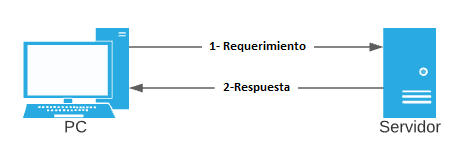
\includegraphics{2.1.png}
      \end{center}
      \caption{Simple comunication method}
   \end{figure}
\end{center}


A client sends an HTTP request to a server in the form of a request
message, beginning with a request-line that includes a method, URI,
and protocol version, followed by header fields
containing request modifiers, client information, and representation
metadata, an empty line to indicate the end of the
header section, and finally a message body containing the payload
body (if any, Section 3.3).
A server responds to a client's request by sending one or more HTTP
   response messages, each beginning with a status line that includes
   the protocol version, a success or error code, and textual reason
   phrase (Section 3.1.2), possibly followed by header fields containing
   server information, resource metadata, and representation metadata
   (Section 3.2), an empty line to indicate the end of the header
   section, and finally a message body containing the payload body (if
   any, Section 3.3).
\subsubsection*{Ejemplo}
The following example illustrates a typical message exchange for a
GET request (Section 4.3.1 of [RFC7231]) on the URI
"http://www.example.com/hello.txt":

Client request:

  GET /hello.txt HTTP/1.1
  User-Agent: curl/7.16.3 libcurl/7.16.3 OpenSSL/0.9.7l zlib/1.2.3
  Host: www.example.com
  Accept-Language: en, mi


Server response:

  HTTP/1.1 200 OK
  Date: Mon, 27 Jul 2009 12:28:53 GMT
  Server: Apache
  Last-Modified: Wed, 22 Jul 2009 19:15:56 GMT
  ETag: "34aa387-d-1568eb00"
  Accept-Ranges: bytes
  Content-Length: 51
  Vary: Accept-Encoding
  Content-Type: text/plain

  Hello World! My payload includes a trailing CRLF.

  HTTP is defined as a stateless protocol, meaning that each request
   message can be understood in isolation.  Many implementations depend
   on HTTP's stateless design in order to reuse proxied connections or
   dynamically load balance requests across multiple servers.  Hence, a
   server MUST NOT assume that two requests on the same connection are
   from the same user agent unless the connection is secured and
   specific to that agent.  Some non-standard HTTP extensions (e.g.,
   [RFC4559]) have been known to violate this requirement, resulting in
   security and interoperability problems.
\subsection{Formato del mensaje (Mejorar intro)}

All HTTP/1.1 messages consist of a start-line followed by a sequence
of octets in a format similar to the Internet Message Format
[RFC5322]: zero or more header fields (collectively referred to as
the "headers" or the "header section"), an empty line indicating the
end of the header section, and an optional message body.
The normal procedure for parsing an HTTP message is to read the
   start-line into a structure, read each header field into a hash table
   by field name until the empty line, and then use the parsed data to
   determine if a message body is expected.  If a message body has been
   indicated, then it is read as a stream until an amount of octets
   equal to the message body length is read or the connection is closed.

 
\subsubsection*{Start Line}
An HTTP message can be either a request from client to server or a
   response from server to client.  Syntactically, the two types of
   message differ only in the start-line, which is either a request-line
   (for requests) or a status-line (for responses), and in the algorithm
   for determining the length of the message body .
   In theory, a client could receive requests and a server could receive
   responses, distinguishing them by their different start-line formats,
   but, in practice, servers are implemented to only expect a request (a
   response is interpreted as an unknown or invalid request method) and
   clients are implemented to only expect a response.

     
   \paragraph*{Request Line}
A request-line begins with a method token, followed by a single space
   (SP), the request-target, another single space (SP), the protocol
   version, and ends with CRLF.

     (podria ir un grafico)

   The method token indicates the request method to be performed on the
   target resource.  The request method is case-sensitive.


   The request-target identifies the target resource upon which to apply
   the request



  
\paragraph*{Status Line}
The first line of a response message is the status-line, consisting
   of the protocol version, a space (SP), the status code, another
   space, a possibly empty textual phrase describing the status code,
   and ending with CRLF.

   (podria ir un grafico)

   The status-code element is a 3-digit integer code describing the
   result of the server's attempt to understand and satisfy the client's
   corresponding request.  The rest of the response message is to be
   interpreted in light of the semantics defined for that status code.
  


\subsubsection* {Header Fields}
Each header field consists of a case-insensitive field name followed
by a colon (":"), optional leading whitespace, the field value, and
optional trailing whitespace.

(podria ir un grafico o con un formato mejor)
header-field   = field-name ":" OWS field-value OWS

The field-name token labels the corresponding field-value as having
the semantics defined by that header field.  

\paragraph*{Field Extensibility}
Header fields are fully extensible: there is no limit on the
introduction of new field names, each presumably defining new
semantics, nor on the number of header fields used in a given
message.  Existing fields are defined in each part of this
specification and in many other specifications outside this document
set.

New header fields can be defined such that, when they are understood
by a recipient, they might override or enhance the interpretation of
previously defined header fields, define preconditions on request
evaluation, or refine the meaning of responses.

\paragraph*{Field Order}
The order in which header fields with differing field names are
   received is not significant.  However, it is good practice to send
   header fields that contain control data first, such as Host on
   requests and Date on responses, so that implementations can decide
   when not to handle a message as early as possible. 


\paragraph*{Whitespace}
This specification uses three rules to denote the use of linear
whitespace: OWS (optional whitespace), RWS (required whitespace), and
BWS ("bad" whitespace).

The OWS rule is used where zero or more linear whitespace octets
might appear.  
The RWS rule is used when at least one linear whitespace octet is
required to separate field tokens.  

The BWS rule is used where the grammar allows optional whitespace
only for historical reasons. 

\paragraph*{Field Parsing}
Messages are parsed using a generic algorithm, independent of the
individual header field names.  The contents within a given field
value are not parsed until a later stage of message interpretation
(usually after the message's entire header section has been
processed).  Consequently, this specification does not use ABNF rules
to define each "Field-Name: Field Value" pair, as was done in
previous editions.  Instead, this specification uses ABNF rules that
are named according to each registered field name, wherein the rule
defines the valid grammar for that field's corresponding field values
(i.e., after the field-value has been extracted from the header
section by a generic field parser).

No whitespace is allowed between the header field-name and colon.  In
the past, differences in the handling of such whitespace have led to
security vulnerabilities in request routing and response handling. 


\paragraph*{Field Limits }
HTTP does not place a predefined limit on the length of each header
field or on the length of the header section as a whole.  Various 
ad hoc limitations on individual header
field length are found in practice, often depending on the specific
field semantics.


\paragraph*{Field Value Components}
(no entiendo, tal vez se puede sacar)
Most HTTP header field values are defined using common syntax
components (token, quoted-string, and comment) separated by
whitespace or specific delimiting characters.  Delimiters are chosen
from the set of US-ASCII visual characters not allowed in a token
%(DQUOTE and "(),/:;<=>?@[\]{}").

  token          = 1*tchar

%  tchar          = "!" / "#" / "$" / "%" / "&" / "'" / "*"
%                 / "+" / "-" / "." / "^" / "_" / "`" / "|" / "~"
                 / DIGIT / ALPHA
                 ; any VCHAR, except delimiters

A string of text is parsed as a single value if it is quoted using
double-quote marks.

  quoted-string  = DQUOTE *( qdtext / quoted-pair ) DQUOTE
  qdtext         = HTAB / SP /%x21 / %x23-5B / %x5D-7E / obs-text
  obs-text       = %x80-FF

Comments can be included in some HTTP header fields by surrounding
the comment text with parentheses.  Comments are only allowed in
fields containing "comment" as part of their field value definition.

  comment        = "(" *( ctext / quoted-pair / comment ) ")"
  ctext          = HTAB / SP / %x21-27 / %x2A-5B / %x5D-7E / obs-text

The backslash octet ("\") can be used as a single-octet quoting
mechanism within quoted-string and comment constructs.  Recipients
that process the value of a quoted-string MUST handle a quoted-pair
as if it were replaced by the octet following the backslash.

  quoted-pair    = "\" ( HTAB / SP / VCHAR / obs-text )

A sender SHOULD NOT generate a quoted-pair in a quoted-string except
where necessary to quote DQUOTE and backslash octets occurring within
that string.  A sender SHOULD NOT generate a quoted-pair in a comment
except where necessary to quote parentheses ["(" and ")"] and
backslash octets occurring within that comment.
\subsubsection*{Message Body }
The message body (if any) of an HTTP message is used to carry the
payload body of that request or response.  The message body is
identical to the payload body unless a transfer coding has been
applied.


The rules for when a message body is allowed in a message differ for
requests and responses.

The presence of a message body in a request is signaled by a
Content-Length or Transfer-Encoding header field.  Request message
framing is independent of method semantics, even if the method does
not define any use for a message body.

The presence of a message body in a response depends on both the
request method to which it is responding and the response status code.  
Responses to the HEAD request method 
never include a message body because the associated
response header fields 
, if present, indicate only what their values would have been if
the request method had been GET (Section 4.3.1 of [RFC7231]). 2xx
(Successful) responses to a CONNECT request method (Section 4.3.6 of
[RFC7231]) switch to tunnel mode instead of having a message body.
All 1xx (Informational), 204 (No Content), and 304 (Not Modified)
responses do not include a message body.  All other responses do
include a message body, although the body might be of zero length.

\paragraph*{Transfer-Encoding }

The Transfer-Encoding header field lists the transfer coding names
corresponding to the sequence of transfer codings that have been (or
will be) applied to the payload body in order to form the message
body.  Transfer codings are defined in Section 4.



Transfer-Encoding is analogous to the Content-Transfer-Encoding field
of MIME, which was designed to enable safe transport of binary data
over a 7-bit transport service .  However, safe
transport has a different focus for an 8bit-clean transfer protocol.
In HTTP's case, Transfer-Encoding is primarily intended to accurately
delimit a dynamically generated payload and to distinguish payload
encodings that are only applied for transport efficiency or security
from those that are characteristics of the selected resource.
. 

For example,

  Transfer-Encoding: gzip, chunked

indicates that the payload body has been compressed using the gzip
coding and then chunked using the chunked coding while forming the
message body.

Unlike Content-Encoding ,
Transfer-Encoding is a property of the message, not of the
representation, and any recipient along the request/response chain
MAY decode the received transfer coding(s) or apply additional
transfer coding(s) to the message body, assuming that corresponding
changes are made to the Transfer-Encoding field-value.  Additional
information about the encoding parameters can be provided by other
header fields not defined by this specification.



Transfer-Encoding was added in HTTP/1.1.  It is generally assumed
that implementations advertising only HTTP/1.0 support will not
understand how to process a transfer-encoded payload. 

\paragraph*{Content-Length }
When a message does not have a Transfer-Encoding header field, a
   Content-Length header field can provide the anticipated size, as a
   decimal number of octets, for a potential payload body.  For messages
   that do include a payload body, the Content-Length field-value
   provides the framing information necessary for determining where the
   body (and message) ends.  For messages that do not include a payload
   body, the Content-Length indicates the size of the selected
   representation .

    

\paragraph*{Message Body Length }

(no entiendo, ver diferencia con content-length)
The length of a message body is determined by one of the following
(in order of precedence):

1.  Any response to a HEAD request and any response with a 1xx
    (Informational), 204 (No Content), or 304 (Not Modified) status
    code is always terminated by the first empty line after the
    header fields, regardless of the header fields present in the
    message, and thus cannot contain a message body.

2.  Any 2xx (Successful) response to a CONNECT request implies that
    the connection will become a tunnel immediately after the empty
    line that concludes the header fields.  A client MUST ignore any
    Content-Length or Transfer-Encoding header fields received in
    such a message.

3.  If a Transfer-Encoding header field is present and the chunked
    transfer coding (Section 4.1) is the final encoding, the message
    body length is determined by reading and decoding the chunked
    data until the transfer coding indicates the data is complete.

    If a Transfer-Encoding header field is present in a response and
    the chunked transfer coding is not the final encoding, the
    message body length is determined by reading the connection until
    it is closed by the server.  If a Transfer-Encoding header field
    is present in a request and the chunked transfer coding is not
    the final encoding, the message body length cannot be determined
    reliably; the server MUST respond with the 400 (Bad Request)
    status code and then close the connection.

    If a message is received with both a Transfer-Encoding and a
    Content-Length header field, the Transfer-Encoding overrides the
    Content-Length.  Such a message might indicate an attempt to
    perform request smuggling (Section 9.5) or response splitting
    (Section 9.4) and ought to be handled as an error.  A sender MUST
    remove the received Content-Length field prior to forwarding such
    a message downstream.

4.  If a message is received without Transfer-Encoding and with
    either multiple Content-Length header fields having differing
    field-values or a single Content-Length header field having an
    invalid value, then the message framing is invalid and the
    recipient MUST treat it as an unrecoverable error.  If this is a
    request message, the server MUST respond with a 400 (Bad Request)
    status code and then close the connection.  If this is a response
    message received by a proxy, the proxy MUST close the connection
    to the server, discard the received response, and send a 502 (Bad
    Gateway) response to the client.  If this is a response message
    received by a user agent, the user agent MUST close the
    connection to the server and discard the received response.

5.  If a valid Content-Length header field is present without
    Transfer-Encoding, its decimal value defines the expected message
    body length in octets.  If the sender closes the connection or
    the recipient times out before the indicated number of octets are
    received, the recipient MUST consider the message to be
    incomplete and close the connection.

6.  If this is a request message and none of the above are true, then
    the message body length is zero (no message body is present).

7.  Otherwise, this is a response message without a declared message
    body length, so the message body length is determined by the
    number of octets received prior to the server closing the
    connection.

Since there is no way to distinguish a successfully completed,
close-delimited message from a partially received message interrupted
by network failure, a server SHOULD generate encoding or
length-delimited messages whenever possible.  The close-delimiting
feature exists primarily for backwards compatibility with HTTP/1.0.

A server MAY reject a request that contains a message body but not a
Content-Length by responding with 411 (Length Required).

Unless a transfer coding other than chunked has been applied, a
client that sends a request containing a message body SHOULD use a
valid Content-Length header field if the message body length is known
in advance, rather than the chunked transfer coding, since some
existing services respond to chunked with a 411 (Length Required)
status code even though they understand the chunked transfer coding.
This is typically because such services are implemented via a gateway
that requires a content-length in advance of being called and the
server is unable or unwilling to buffer the entire request before
processing.

A user agent that sends a request containing a message body MUST send
a valid Content-Length header field if it does not know the server
will handle HTTP/1.1 (or later) requests; such knowledge can be in
the form of specific user configuration or by remembering the version
of a prior received response.

If the final response to the last request on a connection has been
completely received and there remains additional data to read, a user
agent MAY discard the remaining data or attempt to determine if that
data belongs as part of the prior response body, which might be the
case if the prior message's Content-Length value is incorrect.  A
client MUST NOT process, cache, or forward such extra data as a
separate response, since such behavior would be vulnerable to cache
poisoning.


\subsection{Métodos del protocolo HTTP}
4.3.1.  GET

   The GET method requests transfer of a current selected representation
   for the target resource.  GET is the primary mechanism of information
   retrieval and the focus of almost all performance optimizations.
   Hence, when people speak of retrieving some identifiable information
   via HTTP, they are generally referring to making a GET request.

   It is tempting to think of resource identifiers as remote file system
   pathnames and of representations as being a copy of the contents of
   such files.  In fact, that is how many resources are implemented 
   .  However, there are
   no such limitations in practice.  The HTTP interface for a resource
   is just as likely to be implemented as a tree of content objects, a
   programmatic view on various database records, or a gateway to other
   information systems.  Even when the URI mapping mechanism is tied to
   a file system, an origin server might be configured to execute the
   files with the request as input and send the output as the
   representation rather than transfer the files directly.  Regardless,
   only the origin server needs to know how each of its resource
   identifiers corresponds to an implementation and how each
   implementation manages to select and send a current representation of
   the target resource in a response to GET.

  

4.3.2.  HEAD

   The HEAD method is identical to GET except that the server MUST NOT
   send a message body in the response (i.e., the response terminates at
   the end of the header section).  The server SHOULD send the same
   header fields in response to a HEAD request as it would have sent if
   the request had been a GET, except that the payload header fields
    MAY be omitted.  This method can be used for obtaining
   metadata about the selected representation without transferring the
   representation data and is often used for testing hypertext links for
   validity, accessibility, and recent modification.

   

4.3.3.  POST

   The POST method requests that the target resource process the
   representation enclosed in the request according to the resource's
   own specific semantics.  For example, POST is used for the following
   functions (among others):

   o  Providing a block of data, such as the fields entered into an HTML
      form, to a data-handling process;
      o  Posting a message to a bulletin board, newsgroup, mailing list,
      blog, or similar group of articles;

   o  Creating a new resource that has yet to be identified by the
      origin server; and

   o  Appending data to a resource's existing representation(s).

  


   4.3.4.  PUT

   The PUT method requests that the state of the target resource be
   created or replaced with the state defined by the representation
   enclosed in the request message payload.  A successful PUT of a given
   representation would suggest that a subsequent GET on that same
   target resource will result in an equivalent representation being
   sent in a 200 (OK) response.  However, there is no guarantee that 
   such a state change will be observable, since the target resource
   might be acted upon by other user agents in parallel, or might be
   subject to dynamic processing by the origin server, before any
   subsequent GET is received.  A successful response only implies that
   the user agent's intent was achieved at the time of its processing by
   the origin server.


  
    
    4.3.5.  DELETE
    
       The DELETE method requests that the origin server remove the
       association between the target resource and its current
       functionality.  In effect, this method is similar to the rm command
       in UNIX: it expresses a deletion operation on the URI mapping of the
       origin server rather than an expectation that the previously
       associated information be deleted.
    
      
    
       Relatively few resources allow the DELETE method -- its primary use
       is for remote authoring environments, where the user has some
       direction regarding its effect.  For example, a resource that was
       previously created using a PUT request, or identified via the
       Location header field after a 201 (Created) response to a POST
       request, might allow a corresponding DELETE request to undo those
       actions.  Similarly, custom user agent implementations that implement an authoring function, such as revision control clients using HTTP
       for remote operations, might use DELETE based on an assumption that
       the server's URI space has been crafted to correspond to a version
       repository.
    
      
    
    4.3.6.  CONNECT
    
       The CONNECT method requests that the recipient establish a tunnel to
       the destination origin server identified by the request-target and,
       if successful, thereafter restrict its behavior to blind forwarding
       of packets, in both directions, until the tunnel is closed.  Tunnels
       are commonly used to create an end-to-end virtual connection, through
       one or more proxies, which can then be secured using TLS (Transport
       Layer Security, ).
    
       CONNECT is intended only for use in requests to a proxy.  
         However, most origin servers do not implement CONNECT.
     
    
       There are significant risks in establishing a tunnel to arbitrary
       servers, particularly when the destination is a well-known or
       reserved TCP port that is not intended for Web traffic.  For example,
       a CONNECT to a request-target of "example.com:25" would suggest that
       the proxy connect to the reserved port for SMTP traffic; if allowed,
       that could trick the proxy into relaying spam email.  Proxies that
       support CONNECT SHOULD restrict its use to a limited set of known
       ports or a configurable whitelist of safe request targets.
    
    
    4.3.7.  OPTIONS
    
       The OPTIONS method requests information about the communication
       options available for the target resource, at either the origin
       server or an intervening intermediary.  This method allows a client
       to determine the options and/or requirements associated with a
       resource, or the capabilities of a server, without implying a
       resource action.
       An OPTIONS request with an asterisk ("*") as the request-target
    applies to the server in general rather
   than to a specific resource.  Since a server's communication options
   typically depend on the resource, the "*" request is only useful as a
   "ping" or "no-op" type of method; it does nothing beyond allowing the
   client to test the capabilities of the server.  For example, this can
   be used to test a proxy for HTTP/1.1 conformance (or lack thereof).

  
   A server generating a successful response to OPTIONS SHOULD send any
   header fields that might indicate optional features implemented by
   the server and applicable to the target resource (e.g., Allow),
   including potential extensions not defined by this specification.
   The response payload, if any, might also describe the communication
   options in a machine or human-readable representation.  A standard
   format for such a representation is not defined by this
   specification, but might be defined by future extensions to HTTP.  A
   server MUST generate a Content-Length field with a value of "0" if no
   payload body is to be sent in the response.

4.3.8.  TRACE

   The TRACE method requests a remote, application-level loop-back of
   the request message.  The final recipient of the request SHOULD
   reflect the message received, excluding some fields described below,
   back to the client as the message body of a 200 (OK) response with a
   Content-Type of "message/http" .  The
   final recipient is either the origin server or the first server to
   receive a Max-Forwards value of zero (0) in the request
  .

   TRACE allows the client to see what is being received at the other
   end of the request chain and use that data for testing or diagnostic
   information.  The value of the Via header field  is of particular interest, since it acts as a trace of the
   request chain.  Use of the Max-Forwards header field allows the
   client to limit the length of the request chain, which is useful for
   testing a chain of proxies forwarding messages in an infinite loop.



\subsection{Response Status Codes} 
The status-code element is a three-digit integer code giving the
   result of the attempt to understand and satisfy the request.

   HTTP status codes are extensible.  HTTP clients are not required to
   understand the meaning of all registered status codes, though such
   understanding is obviously desirable.  However, a client MUST
   understand the class of any status code, as indicated by the first
   digit, and treat an unrecognized status code as being equivalent to
   the x00 status code of that class, with the exception that a
   recipient MUST NOT cache a response with an unrecognized status code.

   For example, if an unrecognized status code of 471 is received by a
   client, the client can assume that there was something wrong with its
   request and treat the response as if it had received a 400 (Bad
   Request) status code.  The response message will usually contain a
   representation that explains the status.

   The first digit of the status-code defines the class of response.
   The last two digits do not have any categorization role.  There are
   five values for the first digit:

   o  1xx (Informational): The request was received, continuing process

   o  2xx (Successful): The request was successfully received,
      understood, and accepted

   o  3xx (Redirection): Further action needs to be taken in order to
      complete the request

   o  4xx (Client Error): The request contains bad syntax or cannot be
      fulfilled
      o  5xx (Server Error): The server failed to fulfill an apparently
      valid request

\subsection{Overview of Status Codes}

   The status codes listed below are defined in this specification,
   Section 4 of [RFC7232], Section 4 of [RFC7233], and Section 3 of
   [RFC7235].  The reason phrases listed here are only recommendations
   -- they can be replaced by local equivalents without affecting the
   protocol.

   Responses with status codes that are defined as cacheable by default
   (e.g., 200, 203, 204, 206, 300, 301, 404, 405, 410, 414, and 501 in
   this specification) can be reused by a cache with heuristic
   expiration unless otherwise indicated by the method definition or
   explicit cache controls [RFC7234]; all other status codes are not
   cacheable by default.

   \begin{longtable}{|l|l|} 
      \hline
      \textbf{Code} & \textbf{Reason-Phrase}
   \\ \hline 100  & Continue                      
   \\ \hline 101  & Switching Protocols           
   \\ \hline 200  & OK                            
   \\ \hline 201  & Created                       
   \\ \hline 202  & Accepted                      
   \\ \hline 203  & Non-Authoritative Information 
   \\ \hline 204  & No Content                    
   \\ \hline 205  & Reset Content                 
   \\ \hline 206  & Partial Content               
   \\ \hline 300  & Multiple Choices              
   \\ \hline 301  & Moved Permanently             
   \\ \hline 302  & Found                         
   \\ \hline 303  & See Other                     
   \\ \hline 304  & Not Modified                  
   \\ \hline 305  & Use Proxy                     
   \\ \hline 307  & Temporary Redirect            
   \\ \hline 400  & Bad Request                   
   \\ \hline 401  & Unauthorized                  
   \\ \hline 402  & Payment Required              
   \\ \hline 403  & Forbidden                     
   \\ \hline 404  & Not Found                     
   \\ \hline 405  & Method Not Allowed            
   \\ \hline 406  & Not Acceptable                
   \\ \hline 407  & Proxy Authentication Required 
   \\ \hline 408  & Request Timeout               
   \\ \hline 409  & Conflict                      
   \\ \hline 410  & Gone                          
   \\ \hline 411  & Length Required               
   \\ \hline 412  & Precondition Failed           
   \\ \hline 413  & Payload Too Large             
   \\ \hline 414  & URI Too Long                  
   \\ \hline 415  & Unsupported Media Type        
   \\ \hline 416  & Range Not Satisfiable         
   \\ \hline 417  & Expectation Failed            
   \\ \hline 426  & Upgrade Required              
   \\ \hline 500  & Internal Server Error         
   \\ \hline 501  & Not Implemented               
   \\ \hline 502  & Bad Gateway                   
   \\ \hline 503  & Service Unavailable           
   \\ \hline 504  & Gateway Timeout               
   \\ \hline 505  & HTTP Version Not Supported    
   \\ \hline
\end{longtable}

   
   
   \subsubsection*{Informational 1xx}

   The 1xx (Informational) class of status code indicates an interim
   response for communicating connection status or request progress
   prior to completing the requested action and sending a final
   response. 1xx responses are terminated by the first empty line after
   the status-line (the empty line signaling the end of the header
   section).  Since HTTP/1.0 did not define any 1xx status codes, a
   server MUST NOT send a 1xx response to an HTTP/1.0 client.

  


   \subsubsection*{Successful 2xx}

   The 2xx (Successful) class of status code indicates that the client's
   request was successfully received, understood, and accepted.



   \subsubsection*{Redirection 3xx}

   The 3xx (Redirection) class of status code indicates that further
   action needs to be taken by the user agent in order to fulfill the
   request.  If a Location header field (Section 7.1.2) is provided, the
   user agent MAY automatically redirect its request to the URI
   referenced by the Location field value, even if the specific status
   code is not understood.  Automatic redirection needs to done with
   care for methods not known to be safe, as defined in Section 4.2.1,
   since the user might not wish to redirect an unsafe request.

   There are several types of redirects:

   1.  Redirects that indicate the resource might be available at a
       different URI, as provided by the Location field, as in the
       status codes 301 (Moved Permanently), 302 (Found), and 307
       (Temporary Redirect).

   2.  Redirection that offers a choice of matching resources, each
       capable of representing the original request target, as in the
       300 (Multiple Choices) status code.

   3.  Redirection to a different resource, identified by the Location
       field, that can represent an indirect response to the request, as
       in the 303 (See Other) status code.

   4.  Redirection to a previously cached result, as in the 304 (Not
       Modified) status code.



\subsubsection*{Client Error 4xx}

   The 4xx (Client Error) class of status code indicates that the client
   seems to have erred.  Except when responding to a HEAD request, the
   server SHOULD send a representation containing an explanation of the
   error situation, and whether it is a temporary or permanent
   condition.  These status codes are applicable to any request method.
   User agents SHOULD display any included representation to the user.




\subsubsection*{Server Error 5xx}

   The 5xx (Server Error) class of status code indicates that the server
   is aware that it has erred or is incapable of performing the
   requested method.  Except when responding to a HEAD request, the
   server SHOULD send a representation containing an explanation of the
   error situation, and whether it is a temporary or permanent   condition.  A user agent SHOULD display any included representation
   to the user.  These response codes are applicable to any request
   method.

  

\subsection{HTTPS con SSL} 

With an understanding of some of the key concepts of cryptography,
we can now look closely at the operation of the Secure Sockets Layer
(ssl) protocol. Although ssl is not an extremely complicated protocol, 
it does offer several options and variations. 
The ssl protocol consists of a set of messages and rules about when
to send (and not to send) each one. In this chapter, we consider what
those messages are, the general information they contain, and how
systems use the different messages in a communications session. 

\subsubsection*{SSL Roles}
The Secure Sockets Layer protocol defines two different roles for the
communicating parties. One system is always a client, while the other
is a server. The distinction is very important, because ssl requires the
two systems to behave very differently. The client is the system that
initiates the secure communications; the server responds to the client’s request. 
In the most common use of ssl, secure Web browsing,
the Web browser is the ssl client and the Web site is the ssl server.
For ssl itself, the most important distinctions between clients and
servers are their actions during the negotiation of security parameters. 
Since the client initiates a communication, it has the
responsibility of proposing a set of ssl options to use for the
exchange. The server selects from the client’s proposed options,
deciding what the two systems will actually use. Although the final
decision rests with the server, the server can only choose from among
those options that the client originally proposed.

\subsubsection*{SSL Messages}
When ssl clients and servers communicate, they do so by exchanging ssl messages. 
this chapter will show how systems use these messages in their communications.
The most basic function that an ssl client and server can perform is
establishing a channel for encrypted communications. 
This section looks at these steps
in more detail by considering each message in the exchange.


GRAFIQUITO DE LOS MENSAJES 

\paragraph*{ClientHello}
The ClientHello message starts the ssl communication between the
two parties. The client uses this message to ask the server to begin
negotiating security services by using ssl. 

The Version field of the ClientHello message contains the highest
version number of ssl that the client can support. The current ssl
version is 3.0, and it is by far the most widely deployed on the Internet. 

The RandomNumber field, as you might expect, contains a random
number. This random value, along with a similar random value that
the server creates, provides the seed for critical cryptographic calculations.
  The ssl specification suggests that
four of this field’s 32 bytes consist of the time and date. 

The next field in the ClientHello message is SessionID. Although all
ClientHello messages may include this field, in this example, the
field is meaningless and would be empty. 
The CipherSuites field allows a client to list the various cryptographic
services that the client can support, including exact algorithms and
key sizes. The server actually makes the final decision as to which
cryptographic services will be used for the communication, but it is
limited to choosing from this list. 

The CompressionMethods field is, in theory, similar to the CipherSuites field.
 In it, the client may list all of the various data compression methods that 
 it can support. Compression methods are an
important part of ssl because encryption has significant consequences on the 
effectiveness of any data compression techniques. Encryption changes the 
mathematical properties of information in a
way that makes data compression virtually impossible. 

\paragraph*{ServerHello}
When the server receives the ClientHello message, it responds with a
ServerHello. 
The Version field is the first example of a server making a final 
decision for the communications. The ClientHello’s version simply identifies 
which ssl versions the client can support. The ServerHello’s
version, on the other hand, determines the ssl version that the communication
 will use. 
The RandomNumber field of the ServerHello is essentially the same
as in the ClientHello, though this random value is chosen by the
server. Along with the client’s value, this number seeds important
cryptographic calculations. 
The SessionID field of a ServerHello may contain a value, unlike the
ClientHello’s field just discussed. The value in this case uniquely
identifies this particular ssl communication, or session. The main reason for 
explicitly identifying a particular ssl session is to refer to it
again later.
The CipherSuite field (note that the name is singular, not plural, as in
the case of a ClientHello) determines the exact cryptographic parameters, 
specifically algorithms and key sizes, to be used for the session. 
The server must select a single cipher suite from among those
listed by the client in its ClientHello message.
The CompressionMethod field is also singular for a ServerHello. In
theory, the server uses this field to identify the data compression to
be used for the session. Again, the server must pick from among
those listed in the ClientHello. Current ssl versions have not defined
any compression methods, however, so this field has no practical utility.

\paragraph*{ServerKeyExchange}
In this example, the server follows its ServerHello message with a
ServerKeyExchange message. This message complements the CipherSuite field 
of the ServerHello. While the CipherSuite field indicates
the cryptographic algorithms and key sizes, this message contains the
public key information itself. The exact format of the key information depends
 on the particular public key algorithm used. For the rsa
algorithm, for example, the server includes the modulus and public
exponent of the server’s rsa public key.
Note that the ServerKeyExchange message is transmitted without
encryption, so that only public key information can be safely included within it.
 The client will use the server’s public key to encrypt
a session key, which the parties will use to actually encrypt the application
 data for the session.
\paragraph*{ServerHelloDone}
The ServerHelloDone message tells the client that the server has finished with
 its initial negotiation messages. The message itself contains no other 
 information, but it is important to the client, because
once the client receives a ServerHelloDone, it can move to the next
phase of establishing the secure communications.
\paragraph*{ClientKeyExchange}
When the server has finished its part of the initial ssl negotiation,
the client responds with a ClientKeyExchange message. Just as the
ServerKeyExchange provides the key information for the server, the
ClientKeyExchange tells the server the client’s key information. In

this case, however, the key information is for the symmetric encryption 
algorithm both parties will use for the session. Furthermore, the
information in the client’s message is encrypted using the public key
of the server. This encryption protects the key information as it traverses
 the network, and it allows the client to verify that the server
truly possesses the private key corresponding to its public key. Otherwise,
 the server won’t be able to decrypt this message. This operation is an 
 important protection against an attacker that intercepts
messages from a legitimate server and pretends to be that server by
forwarding the messages to an unsuspecting client. Since a fake
server won’t know the real server’s private key, it won’t be able to decrypt 
the ClientKeyExchange message. Without the information in
that message, communication between the two parties cannot succeed.
\paragraph*{ChangeCipherSpec}
After the client sends key information in a ClientKeyExchange message, 
the preliminary ssl negotiation is complete. At that point, the
parties are ready to begin using the security services they have negotiated.
 The ssl protocol defines a special message—
ChangeCipherSpec—to explicitly indicate that the security services
should now be invoked.
Since the transition to secured communication is critical, and both
parties have to get it exactly right, the ssl specification is very precise
in describing the process. First, it identifies the set of information
that defines security services. That information includes a specific
symmetric encryption algorithm, a specific message integrity algorithm, 
and specific key material for those algorithms. The ssl specification also 
recognizes that some of that information (in particular,
the key material) will be different for each direction of communication. 
In other words, one set of keys will secure data the client sends
to the server, and a different set of keys will secure data the server
sends to the client. (In principle, the actual algorithms could differ as
well, but ssl does not define a way to negotiate such an option.) For
any given system, whether it is a client or a server, ssl defines a write
state and a read state. The write state defines the security information

for data that the system sends, and the read state defines the security
information for data that the system receives.
The ChangeCipherSpec message serves as the cue for a system to
begin using its security information. Before a client or server sends a
ChangeCipherSpec message, it must know the complete security information it 
is about to activate. As soon as the system sends this
message, it activates its write state. Similarly, as soon as a system receives
 a ChangeCipherSpec from its peer, the system activates its
read state.

GRAFIQUITO Figures 3-2 and 3-3

\paragraph*{Finished}
Immediately after sending their ChangeCipherSpec messages, each
system also sends a Finished message. The Finished messages allow
both systems to verify that the negotiation has been successful and
that security has not been compromised. Two aspects of the Finished
message contribute to this security. First, as the previous subsection
explained, the Finished message itself is subject to the negotiated cipher suite. 
That means that it is encrypted and authenticated according to that suite.
 If the receiving party cannot successfully decrypt
and verify the message, then clearly something has gone awry with
the security negotiation.
The contents of the Finished message also serve to protect the security of the
 ssl negotiation. Each Finished message contains a cryptographic hash of 
 important information about the just-finished
negotiation.  Notice that protected data includes the exact content of all
handshake messages used in the exchange (though ChangeCipherSpec messages 
are not considered “handshake” messages in the strict
sense of the word, and thus are not included). This protects against
an attacker who manages to insert fictitious messages or remove 
legitimate messages from the communication. If an attacker were able
to do so, the client’s and server’s hash calculations would not match,
and they would detect the compromise.

\paragraph*{Ending Secure Communications}

Although as a practical matter it is rarely used (primarily due to the
nature of Web sessions), ssl does have a defined procedure for ending a
 secure communication between two parties. In this procedure,
 the two systems each send a special ClosureAlert to the other.
Explicitly closing a session protects against a truncation attack, in
which an attacker is able to compromise security by prematurely terminating
 a communication. 

\subsubsection*{Authenticating the Server’s Identity}
previously it was explained how ssl can establish encrypted
communications between two parties, that may not really add that
much security to the communication. With encryption alone neither
party can really be sure of the other’s identity. The typical reason for
using encryption in the first place is to keep information secret from
some third party. But if that third party were able to successfully
masquerade as the intended recipient of the information, then encryption 
would serve no purpose. The data would be encrypted, but
the attacker would have all the data necessary to decrypt it.
To avoid this type of attack, ssl includes mechanisms that allow each
party to authenticate the identity of the other. With these mechanisms, 
each party can be sure that the other is genuine, and not a
masquerading attacker. In this section, we’ll look at how ssl enables a
server to authenticate itself.
A natural question is, of course, if authenticating identities is so important,
 why don’t we always authenticate both parties? 
 Aca un ejemplo que sirva en una red interna
 The answer
lies in the nature of Web commerce. When you want to purchase
something using your Web browser, it’s very important that the Web
site you’re browsing is authentic. You wouldn’t want to send your
credit card number to some imposter posing as your favorite merchant. 
The merchant, on the other hand, has other means for
authenticating your identity. Once it receives a credit card number,
for example, it can validate that number. Since the server doesn’t
need ssl to authenticate your identity, the ssl protocol allows for
server authentication only. 

\paragraph*{Certificate}
When authenticating your identity, the server sends a Certificate message 
in place of the ServerKeyExchange message previously described. The Certificate 
message simply contains a certificate chain
that begins with the server’s public key certificate and ends with the
certificate authority’s root certificate.
The client has the responsibility to make sure it can trust the certificate it 
receives from the server. That responsibility includes verifying
the certificate signatures, validity times, and revocation status. It also
means ensuring that the certificate authority is one that the client
trusts. Typically, clients make this determination by knowing the
public key of trusted certificate authorities in advance, through some
trusted means. Netscape and Microsoft, for example, preload their
browser software with public keys for well-known certificate authorities. 
Web servers that want to rely on this trust mechanism can only
obtain their certificates (at least indirectly) from one of these wellknown
 authorities.

\paragraph*{ClientKeyExchange}
The client’s ClientKeyExchange message also differs in server authentication, 
though the difference is not major. When encryption
only is to be used, the client encrypts the information in the ClientKeyExchange
 using the public key the server provides in its
ServerKeyExchange message. In this case, of course, the server is authenticating
 itself and, thus, has sent a Certificate message instead of
a ServerKeyExchange. The client, therefore, encrypts its ClientKeyExchange information 
using the public key contained in the
server’s certificate. This step is important because it allows the client
to make sure that the party with whom it is communicating actually
possesses the server’s private key. Only a system with the actual private key will 
be able to decrypt this message and successfully continue the communication.

\subsubsection*{Certificate Functionality}

\paragraph*{Single Domain}
As the name suggests, a single domain SSL certificate can only be used on a single 
domain or IP. This is considered the default SSL certificate type. The DV SSL type is
available at all validation levels.
\paragraph*{Multi-Domain}
This SSL type is a jack-of-all-trades certificate. Multi-Domain Wildcards can encrypt
 up to 250 different domains and unlimited sub-domains. Unfortunately, it's not available
  in EV.
\paragraph*{Wildcard}
Wildcards are specifically designed to encrypt one domain and all of its accompanying 
sub-domains. Unlimited sub-domains. Unfortunately, Wildcards are only available at the 
DV and OV levels.
\paragraph*{Multi-Domain Wildcard}
These are the jack-of-all-trades certificates. Multi-Domain Wildcards can encrypt up 
to 250 different domains and unlimited sub-domains. Unfortunately, it's not available 
in EV.

\subsubsection*{Validation Level}
There are three types of SSL Certificate available today; Extended Validation 
(EV SSL), Organization Validated (OV SSL) and Domain Validated (DV SSL). The 
encryption levels are the same for each certificate, what differs is the vetting
 and verification processes needed to obtain the certificate.
\paragraph*{Domain Validation (DV)}
Domain Validation SSL or DV SSL represents the base-level for SSL types. These 
are perfect for websites that just need encryption and nothing more. DV SSL 
certificates are typically inexpensive and they can be issued within minutes. That's 
because the validation process is fully automated. Just prove you own your domain 
and the DV SSL certificate is yours.
\paragraph*{Organization Validation (OV)}
Organization Validation SSL or OV SSL represents the middle ground for SSL certificate 
types. To obtains OV SSL, your company or organization must undergo light business
 vetting. This can take up to three business days because someone has to verify 
 your business information. OV SSL displays the same visual indicators as DV SSL,
  but provides a way for your customers to check your verified business information 
  in the certificate details section.
\paragraph*{Extended Validation (EV)}
Extended Validation SSL or EV SSL requires extensive business vetting by Comodo. This
 may sound like a lot, but it's really not if your business has publicly available 
 records. EV SSL activates a unique visual indicator – your verified organization name
  shown in the browser.

  
\subsubsection*{Identifier Validation Challenges}

(CAMBIAR LA INTRO, NO ME GUSTA LO DE IDENTIFICADOR, RELACIONARLO MAS CON UN DOMINIO)

ACME uses an extensible challenge/response framework for identifier
validation.  The server presents a set of challenges in the
authorization object it sends to a client (as objects in the
"challenges" array), and the client responds by sending a response
object in a POST request to a challenge URL.

   Different challenges allow the server to obtain proof of different
   aspects of control over an identifier.  In some challenges, like HTTP
   and DNS, the client directly proves its ability to do certain things
   related to the identifier.  The choice of which challenges to offer
   to a client under which circumstances is a matter of server policy.


   

\paragraph*{HTTP Challenge}

   With HTTP validation, the client in an ACME transaction proves its
   control over a domain name by proving that it can provision HTTP
   resources on a server accessible under that domain name.  The ACME
   server challenges the client to provision a file at a specific path,
   with a specific string as its content.

   This is the most common challenge type today. The server gives a
   token to your ACME client, and your ACME client puts a file on your web 
   server at {http://\<YOUR\_DOMAIN\>/.well-known/acme-challenge/\<TOKEN\>}. That 
   file contains the token, plus a thumbprint of your account key. 

   Once the client tells to the server that the file is ready, the server 
   tries retrieving it.On receiving a response, the server constructs and stores the key
   authorization from the challenge "token" value and the current client
   account key.

   Given a challenge/response pair, the server verifies the client's
   control of the domain by verifying that the resource was provisioned
   as expected.

   (TAL VEZ PARA LA PRESENTACION)

   Pros:

    It’s easy to automate without extra knowledge about a domain’s configuration.
    It allows hosting providers to issue certificates for domains CNAMEd to them.
    It works with off-the-shelf web servers.

   Cons:

    It doesn’t work if your ISP blocks port 80 (this is rare, but some residential ISPs do this).
    Let’s Encrypt doesn’t let you use this challenge to issue wildcard certificates.
    If you have multiple web servers, you have to make sure the file is available on all of them.

   (EXPLICAR POR QUE NO PUEDO USAR ESTE DESAFIO)

\paragraph*{DNS Challenge}
   When the identifier being validated is a domain name, the client can
   prove control of that domain by provisioning a TXT resource record
   containing a designated value for a specific validation domain name.

   A client fulfills this challenge by constructing a key authorization
   from the "token" value provided in the challenge and the client's
   account key.  The client then computes the SHA-256 digest 
   of the key authorization.

   The record provisioned to the DNS contains the base64url encoding of
   this digest.  The client constructs the validation domain name by
   prepending the label {\_acme-challenge} to the domain name being
   validated, then provisions a TXT record with the digest value under
   that name.  For example, if the domain name being validated is
   "www.example.org", then the client would provision the following DNS
   record:
   \_acme-challenge.www.example.org. 300 IN TXT "gfj9Xq...Rg85nM"
   
   On receiving a response, the server constructs and stores the key
   authorization from the challenge "token" value and the current client
   account key.

   To validate a DNS challenge, the server performs the following steps:

   1.  Compute the SHA-256 digest of the stored key
       authorization

   2.  Query for TXT records for the validation domain name

   3.  Verify that the contents of one of the TXT records match the
       digest value

   If all of the above verifications succeed, then the validation is
   successful.  If no DNS record is found, or DNS record and response
   payload do not pass these checks, then the validation fails.

   The client SHOULD de-provision the resource record(s) provisioned for
   this challenge once the challenge is complete, i.e., once the
   "status" field of the challenge has the value "valid" or "invalid".
